\chapter{Conceptos Fundamentales}

\section{Gr\'aficas}

Esta secci\'on y la siguiente (\ref{section:arboles}) fueron basadas en \citetitle{open}\cite{open}

\begin{definition}[Gr\'afica]
Una \textbf{gr\'afica} es un par ordenado $G=(V, E)$ que consiste de un conjunto no vac\'io $V$ (llamado v\'ertices) y un conjunto $E$ (llamado aristas) formado por duplas de elementos de $V$.\ref{fig:graph}
\end{definition}

\begin{figure}
\centering
  \begin{tikzpicture} [every node/.style={circle, draw, fill=blue!20}]
    %\draw[help lines] (0,0) grid (4,-2);
    \node (h) at (2,-2) {h};
    \graph {
      a -- {
        b -- c,
        d -- e -- f -- g
      };
      d -- (h) --[bend left] f;
      b -- d;
      c -- e;
      e -- i;
    };
  \end{tikzpicture}
  \caption{Una gr\'afica conexa $G$.}\label{fig:graph}
\end{figure}

\begin{definition}[Adyacencia]
La \textbf{adyacencia} se define de forma distinta para v\'ertices que para aristas. Dos v\'ertices son adyacentes si estan conectados por una arista. Dos aristas son adyacentes si comparten un v\'ertice.
\end{definition}

\begin{definition}[Recorrido]
Un \textbf{recorrido} es una secuencia de v\'ertices tal que, v\'ertices consecutivos en dicha secuencia son adyacentes en la gr\'afica.
\end{definition}

\begin{definition}[Camino]
Un \textbf{camino} es un recorrido que no repite v\'ertices (o aristas) excepto, tal vez, el primero y el \'ultimo. Si un camino empieza y termina en el mismo v\'ertice, se llama \textbf{ciclo}.
\end{definition}

\begin{figure}
\centering
  \begin{subfigure}{0.4\textwidth}
  \begin{tikzpicture} [every node/.style={circle, draw, fill=blue!20}]
    %\draw[help lines] (0,0) grid (4,-2);
    \node[fill=red!20] (h) at (2,-2) {h};
    \graph {
      a -- {
        b[fill=red!20] -- c,
        d[fill=red!20] --[red, thick] e[fill=red!20] --[red, thick] f[fill=red!20] -- g
      };
      d -- (h) --[red, thick] f;
      b[fill=red!20] --[red, thick] d;
      c -- e;
    };
  \end{tikzpicture}
  \caption{Un camino (en rojo) en $G$.}\label{fig:graph}
  \end{subfigure}
  \begin{subfigure}{0.4\textwidth}
  \begin{tikzpicture} [every node/.style={circle, draw, fill=blue!20}]
    %\draw[help lines] (0,0) grid (4,-2);
    \node (h) at (2,-2) {h};
    \graph {
      a -- {
        b[fill=green!20] --[green, thick] c[fill=green!20],
        d[fill=green!20] --[green, thick] e[fill=green!20] -- f -- g
      };
      d -- (h) -- f;
      b --[green, thick] d;
      c --[green, thick] e;
    };
  \end{tikzpicture}
  \caption{Un ciclo (en verde) en $G$.}\label{fig:graph}
  \end{subfigure}
\end{figure}

Cuando dos gr\'aficas son b\'asicamente la misma, pero no necesariamente iguales, son llamadas \emph{isomorfas}. La definici\'on de isomorfismo es como sigue:

\begin{definition}[Isomorfismo]
Un \textbf{isomorfismo} entre dos gr\'aficas $G_1$ y $G_2$ es una biyecci\'on $f: V_1 \to V_2$ entre los v\'ertices de las gr\'aficas tal que $\{a,b\}$ es una arista en $G_1$ si, y solo si, $\{f(a), f(b)\}$ es una arista en $G_2$.
\end{definition}

\begin{figure}
\centering
  \begin{subfigure}{0.4\textwidth}
  \begin{tikzpicture} [every node/.style={circle, draw, fill=red!20}]
    \graph [simple necklace layout] {
      a -- {
        b -- c,
        d -- e -- f -- g
      };
    };
  \end{tikzpicture}
  \caption{Gr\'afica $G'$}
  \end{subfigure}
  \begin{subfigure}{0.4\textwidth}
  \begin{tikzpicture} [every node/.style={rectangle, draw, fill=green!20}]
    \graph {
      1 -- {
        2 -- 3,
        4 -- 5 -- 6 -- 7
      };
    };
  \end{tikzpicture}
  \caption{Gr\'afica $H'$}
  \end{subfigure}
  \caption{Isomorfismo entre $G'$ y $H'$.}\label{fig:graph}
\end{figure}

Dos gr\'aficas son isomorfas si existe un isomorfismo entre ellas. En ese caso escribimos $G_1\cong G_2$

\begin{definition}[Subgr\'afica]
Decimos que $G' = (V', E')$ es una \textbf{subgr\'afica} de $G=(V,E)$, y escribimos $G'\subseteq G$, si se cumple que $V'\subseteq V$ y que $E'\subseteq E$.
\end{definition}
\begin{figure}
\centering
  \begin{tikzpicture} [every node/.style={circle, draw, fill=blue!20}]
    \graph {
        d -- e; f -- g;
    };
  \end{tikzpicture}
  \caption{Una subgr\'afica de $G$. No inducida, pues la arista $(e,f)$ no aparece.}\label{fig:graph}
\end{figure}

\begin{definition}[Subgr\'afica inducida]
Decimos que $G' = (V', E')$ es una \textbf{subgr\'afica inducida} de $G=(V,E)$ si se cumple que $V'\subseteq V$ y que cada arista en $E$ cuyos v\'ertices siguen estando en $V'$ tambi\'en es una arista en $E'$.
\end{definition}
\begin{figure}
\centering
  \begin{tikzpicture} [every node/.style={circle, draw, fill=blue!20}]
    \graph {
        d -- e -- f -- g;
    };
  \end{tikzpicture}
  \caption{Una subgr\'afica inducidad de $G$.}\label{fig:graph}
\end{figure}

\begin{definition}[Gr\'afica conexa]
Una gr\'afica es \textbf{conexa} cuando podemos llegar de cualquier v\'ertice a cualquier otro v\'ertice siguiendo alg\'un camino de aristas.
\end{definition}

\begin{definition}[Grado de un v\'ertice]
Al n\'umero de aristas que emanan de un v\'ertice dado le llamamos el \textbf{grado} de ese v\'ertice. El m\'aximo (o el m\'inimo) grado \emph{de una gr\'afica} hace referencia al m\'aximo (o el m\'inimo) grado de sus v\'ertices.
\end{definition}

\begin{definition}[Gr\'afica plana]
Cuando una gr\'afica \textit{puede} ser dibujada en el plano sin que ninguna de sus aristas se crucen, se dice que es \textbf{plana}.
\end{definition}

\begin{figure}
  \begin{tikzpicture}
    \graph [clockwise] { subgraph K_n [n=5] };
  \end{tikzpicture}
  \caption{Grafica plana, no representada en su forma plana.}
\end{figure}

\subsection{\'Arboles}
\label{section:arboles}

\begin{definition}[\'Arbol]
Un \textbf{\'arbol} es una gr\'afica \emph{conexa} y que no contiene \emph{ciclos}.
\end{definition}

Cuando designamos un nodo como \emph{ra\'iz}, todos los dem\'as v\'ertices en el \'arbol pueden ser identificados por su posici\'on relativa a la ra\'iz. Esto es debido a que existe un \'unico camino entre cualesquiera dos v\'ertices en un \'arbol.

Si dos vértices son adyacentes, decimos que uno de ellos es el \textbf{padre} del otro, el cual es llamado \textbf{hijo}. De los dos, el padre es el que se encuentra m\'as cerca de la r\'aiz. Por lo tanto la ra\'iz del \'arbol es un padre pero no es el hijo de ning\'un v\'ertice.

As\'i mismo, el hijo de el hijo de un v\'ertice es el \textbf{nieto} de ese v\'ertice (convirti\'endose en \textbf{abuelo}). Generalizando, decimos que un v\'ertice $v$ es \textbf{descendiente} de un v\'ertice $u$ si $u$ es un v\'ertice en el camino de $v$ a la ra\'iz. Entonces, llamaremos a $u$, un \textbf{ancestro} de $v$.

El propósito de este lenguaje es ayudarnos a recorrer el árbol. Recorrer el árbol, visitando cada nodo en algún orden, es un paso escencial en muchos algoritmos. Cuando visitamos primero todos los vértices de una misma generación antes de visitar la siguiente, decimos que hacemos una \textbf{b\'usqueda a lo ancho} (en inglés BFS o \textit{Breadth First Search}). Por otro lado, cuando primero viajamos a lo más alejado posible de la raíz, y luego retrocedemos hasta una disyunción y poder viajar hacia adelante otra vez, le llamamos \textbf{b\'usqueda en profundidad} (en inglés DFS o \textit{Depth First Search}). Decimos ``b\'usqueda'' porque la mayoría de las veces recorremos el árbol tratando de encontrar vértices con cierta propiedad.

\begin{definition}[\'Arbol generador]
Dada una gr\'afica conexa $G$, un \textbf{\'arbol generador} de $G$ es una subgr\'afica de $G$ que es un \'arbol y que contiene todos los v\'ertices de $G$. Todas las gr\'aficas conexas tienen \'arbol generador.
\end{definition}

\begin{figure}
\centering
  \begin{subfigure}{0.4\textwidth}
    \begin{tikzpicture} [every node/.style={circle, draw, fill=blue!20}]
      %\draw[help lines] (0,0) grid (4,-2);
      \node (h) at (2,-2) {h};
      \graph {
        a -- b -- c;
        d   -- e -- f -- g;
        (h) -- g;
        c -- e;
      };
    \end{tikzpicture}
    \caption{Un \'arbol generador de $G$.}\label{fig:graph}
  \end{subfigure}
  \begin{subfigure}{0.4\textwidth}
    \begin{tikzpicture} [every node/.style={circle, draw, fill=blue!20}]
      %\draw[help lines] (0,0) grid (4,-2);
      \node (h) at (2,-2) {h};
      \graph {
        a -- {
          b -- c,
          d -- e -- f -- g
        };
        d -- (h);
      };
    \end{tikzpicture}
    \caption{Otro \'arbol generador de $G$.}
  \end{subfigure}
  \caption{\'Arbol generador}
\end{figure}

\section{Gr\'aficas geom\'etricas}

\begin{definition}[Gr\'afica geom\'etrica]
Una gr\'afica es \textbf{geom\'etrica} cuando es dibujada en el plano (no necesariamente es plana) utilizando segmentos (parte de una l\'inea, definido por dos puntos), y ning\'una tercia de v\'ertices yacen sobre la misma l\'inea recta, es decir que no son \emph{colineales}. \cite{handbook}
\end{definition}

Aunque la definición de gráfica plana es muy similar, vale la pena denotar las diferencias: la planaridad es la cualidad de una gŕafica de \textit{poder} ser dibujada sin que sus aristas se crucen, mientras que una gráfica geométrica necesariamente está representada en el plano.

Las siguientes definiciones fueron basadas en \citetitle{tamassia}\cite{tamassia}, excepto donde se indique lo contrario.

\begin{definition}[Gr\'afica de plano]
Una \textbf{gr\'afica de plano}, $G=(V, E)$ es una gr\'afica geom\'etrica como la definida anteriormente salvo dos diferencias; el conjunto de aristas $E$ es un conjunto de curvas simples que conectan dos v\'ertices en $V$ y, las curvas simples de $E$ no se cruzan entre ellas, excepto, posiblemente, en los extremos. Una gr\'afica de plano divide al conjunto de puntos en el plano que no pertenecen a las aristas en regiones conectadas topológicamente, llamadas \emph{caras}. La región no acotada es llamada \emph{cara externa}. Una gr\'afica es planar si es isomorfa a alguna gr\'afica de plano.
\end{definition}

\begin{figure}
  \begin{tikzpicture}
    \begin{scope} [every node/.style={circle, draw, fill=blue!20}]
      \node (a) at (2, 0) {a};
      \node (b) at (0, -1) {b};
      \node (c) at (1.5, -1.5) {c};
      \node (d) at (0.5, -3) {d};
      \node (e) at (3.5, -2.5) {e};
      \graph {
        (b) -- {(a), (c), (d)};
        (c) -- {(a), (d)};
        (a) --[bend left] (e);
        (d) --[bend right] (e);
      };
    \end{scope}
    \begin{scope}
      \node (f1) at (2.3, -2) {$f_1$};
      \node (f2) at (1.3, -0.75) {$f_2$};
      \node (f3) at (0.6, -1.9) {$f_3$};
      \node (fe) at (3.5, -0.6) {$f_e$};
      \graph {
        (f1);
        (f2);
        (f3);
        (fe);
      };
    \end{scope}
  \end{tikzpicture}
  \caption{Gr\'afica de plano}
\end{figure}

\begin{definition}[Representaci\'on planar]
Le llamaremos \textbf{representaci\'on planar} al conjunto de listas ordenadas de aristas $P(f)$, una por cada cara $f$, que describen la estructura topol\'ogica de la gr\'afica al listar las aristas que aparecen en el contorno de cada cara, y especificando la cara externa.
\end{definition}

\begin{definition}[Gr\'afica ortogonal]
Una \textbf{gr\'afica ortogonal} es una gr\'afica de plano cuyas aristas son secuencias alternantes de segmentos horizontales y verticales. La \emph{representacion ortogonal} describe la forma de una gr\'afica ortogonal, sin considerar la longitud de los segmentos.
\end{definition}

\begin{figure}
  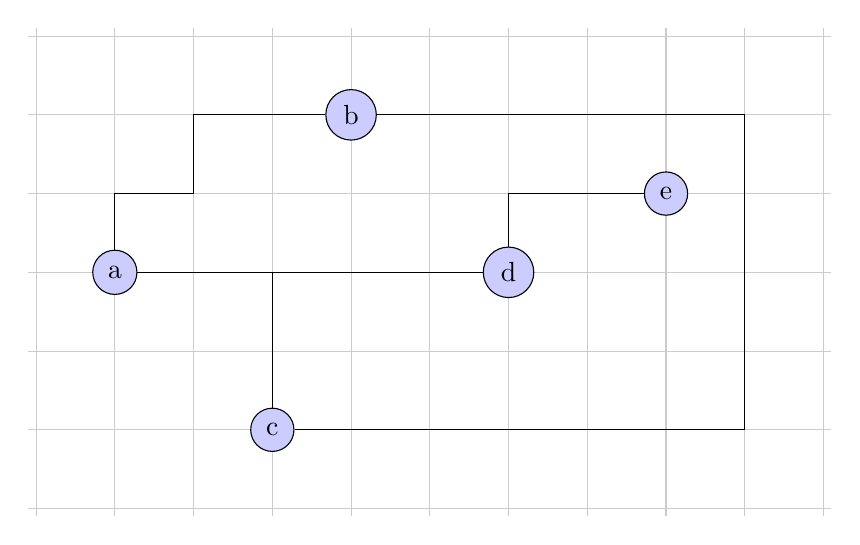
\begin{tikzpicture} [every node/.style={circle, draw, fill=blue!20}]
    \draw[black!20, thin] (-0.1,-0.1) grid (10.1,6.1);
    \node (a) at (1, 3) {a};
    \node (b) at (4, 5) {b};
    \node (c) at (3, 1) {c};
    \node (d) at (6, 3) {d};
    \node (e) at (8, 4) {e};
    \draw (a) -- (1,4) -- (2,4) -- (2,5) -- (b);
    \draw (a) -- (d);
    \draw (3,3) -- (c);
    \draw (d) -- (6, 4) -- (e);
    \draw (b) -- (9,5) -- (9,1) -- (c);
  \end{tikzpicture}
  \caption{Gr\'afica ortogonal}
\end{figure}

\begin{definition}[Malla rectilinea]
La \textbf{malla rectilinea} o \textbf{malla ortogonal} es la gr\'afica planar infinita cuyos v\'ertices (o puntos) tienen coordenadas enteras, y cuyas aristas ligan a cada par de v\'ertices que se encuentran a distancia unitaria. Un \textbf{encajamiento planar} en la malla $M = (V_M, E_M)$, de una gr\'afica $G = (V, M)$ es una correspondencia $Q: G\mapsto M$ que cumple que: (1) $Q$ mapea cada v\'ertice en $G$ a una posici\'on distinta de la malla; (2) $Q$ mapea cada arista $e$ de $G$ a un camino en la malla $Q(e)$ cuyos extremos son mapeos de v\'ertices ligados por $e$; (3) Los caminos $Q(e')$ y $Q(e'')$ correspondientes a cada par de aristas $\{e', e''\}$ de $G$, no tienen puntos en com\'un, excepto, tal vez, los extremos.
\end{definition}

\begin{figure}
  \begin{subfigure}{0.3\textwidth}
    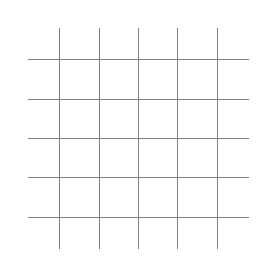
\begin{tikzpicture}
      \draw[step=.5cm, thin, gray] (-1.4,-1.4) grid (1.4,1.4);
    \end{tikzpicture}
    \caption{Rectil\'inea}
  \end{subfigure}
  \begin{subfigure}{0.3\textwidth}
    \begin{tikzpicture}[hexa/.style= {shape=regular polygon, regular polygon sides=6, minimum size=0.5cm, draw,anchor=south, thin, gray}]
      \foreach \j in {0,...,4}{%
         \ifodd\j
             \foreach \i in {0,...,4}{\node[hexa] (h\j;\i) at ({\j/4+\j/8},{((\i+1/2)*sin(60))/2}) {};}
        \else
             \foreach \i in {0,...,4}{\node[hexa] (h\j;\i) at ({\j/4+\j/8},{(\i*sin(60))/2}) {};}
        \fi}
    \end{tikzpicture}
    \caption{Hexagonal}
  \end{subfigure}
  \begin{subfigure}{0.3\textwidth}
    \begin{tikzpicture}[scale=0.5]
      \coordinate (0;0) at (0,0);

      \foreach \c in {1,...,3}{%
        \foreach \i in {0,...,5}{%
          \pgfmathtruncatemacro\j{\c*\i}
          \coordinate (\c;\j) at (60*\i:\c);
        }
      }
      \foreach \i in {0,2,...,10}{%
        \pgfmathtruncatemacro\j{mod(\i+2,12)}
        \pgfmathtruncatemacro\k{\i+1}
        \coordinate (2;\k) at ($(2;\i)!.5!(2;\j)$);
      }
      \foreach \i in {0,3,...,15}{%
        \pgfmathtruncatemacro\j{mod(\i+3,18)}
        \pgfmathtruncatemacro\k{\i+1}
        \pgfmathtruncatemacro\l{\i+2}
        \coordinate (3;\k) at ($(3;\i)!1/3!(3;\j)$);
        \coordinate (3;\l) at ($(3;\i)!2/3!(3;\j)$);
      }

      \foreach \i in {0,...,6}{%
        \pgfmathtruncatemacro\k{\i}
        \pgfmathtruncatemacro\l{15-\i}
        \draw[thin,gray] (3;\k)--(3;\l);

        \pgfmathtruncatemacro\k{9-\i}
        \pgfmathtruncatemacro\l{mod(12+\i,18)}
        \draw[thin,gray] (3;\k)--(3;\l);

        \pgfmathtruncatemacro\k{12-\i}
        \pgfmathtruncatemacro\l{mod(15+\i,18)}
        \draw[thin,gray] (3;\k)--(3;\l);
      }
    \end{tikzpicture}
    \caption{Triangular}
  \end{subfigure}
  \caption{Mallas}
\end{figure}

\begin{figure}
  \begin{subfigure}{0.5\textwidth}
    \begin{tikzpicture}[every node/.style={circle, draw, fill=blue!20, radius=0.3cm}]
      \graph [spring layout, node distance=1.2cm, coarsen] {
        a -- {b,c,d};
        b -- {d,f};
        c -- {f,e};
        e -- {f,g,h};
        g -- {h,k,i};
        k[x=2] -- i;
      };
    \end{tikzpicture}
    \caption{G}
  \end{subfigure}
  \begin{subfigure}{0.4\textwidth}
    \begin{tikzpicture}[scale=0.6, every node/.style={circle, draw, fill=blue!20, radius=0.3cm}]
      \draw[black!20, thin] (-0.3,-0.3) grid (10.3,5.3);
      \node (a) at (0,2) {a};
      \node (b) at (2,0) {b};
      \node (c) at (0,4) {c};
      \node (d) at (0,0) {d};
      \node (e) at (6,2) {e};
      \node (f) at (4,2) {f};
      \node (g) at (8,2) {g};
      \node (h) at (6,0) {h};
      \node (i) at (8,4) {i};
      \node (k) at (10,2) {k};
      \coordinate (ab) at (2,2) {};
      \coordinate (bf) at (4,0) {};
      \coordinate (hg) at (8,0) {};
      \coordinate (ki) at (10,4) {};
      \coordinate (cf) at (4,4) {};
      \coordinate (ce) at (0,5) {};
      \coordinate (cx) at (6,5) {};
      \graph {
        (e) -- {
          (cx) -- (ce) -- (c),
          (g) -- {
            (k) -- (ki) -- (i), (i)
          },
          (h) -- (hg) -- (g),
          (f) -- {
            (cf) -- (c),
            (bf) -- (b) -- {
              (ab) -- (a),
              (d) -- (a) -- (c)
            }
          }
        },
        (g) -- (e)
      };
    \end{tikzpicture}
    \caption{Q(G)}
  \end{subfigure}
  \caption{Encajamiento en la malla}
\end{figure}

La gr\'afica planar $Q(G)$ definida por el encajamiento (o incrustamiento) $Q$ es isomorfa a $G$. Una gr\'afica admite ser incrustada en la malla si, y solo si, es planar y sus v\'ertices tienen un grado m\'aximo menor o igual 4. Para acortar, nos referiremos a estas graficas como \emph{4-planares}.

\begin{definition}[Doblez]
Contamos un \emph{doblez}\cite{minbends} por cada par de aristas consecutivas en una gr\'afica ortogonal que no yacen sobre la misma l\'inea.
\end{definition}

\begin{figure}
  \begin{subfigure}{0.4\textwidth}
    \begin{tikzpicture} [every node/.style={circle, draw, fill=blue!20}]
      \graph {a -- b -- c};
    \end{tikzpicture}
    \caption{No hay doblez entre $a$ y $c$}
  \end{subfigure}
  \begin{subfigure}{0.4\textwidth}
    \begin{tikzpicture} [every node/.style={circle, draw, fill=blue!20}]
      \graph {a -- b -- c[x=-1, y=1]};
    \end{tikzpicture}
    \caption{S\'i hay doblez entre $a$ y $c$}
  \end{subfigure}
  \caption{Doblez}
\end{figure}

\begin{definition}[Modelo en l\'inea recta]
Un \textbf{modelo en l\'inea recta}\cite{minbends}, o \textbf{s-modelo}, \footnote{Del ingl\'es: \textit{straight model}, cuya traducci\'on propiamente ser\'ia modelo-rl} se refiere a la gr\'afica ortogonal que resulta del encajamiento planar de un \'arbol en la malla. Como podemos ver en las figuras correspondientes, un arbol puede ser encajado sin dobleces en las aristas que no incluyen otro nodo del arbol, es decir que todas las aristas se mapean a caminos rectos.
\end{definition}

\begin{figure}
  \begin{tikzpicture}
    \begin{scope}[every node/.style={circle, draw, fill=blue!20}]
      \graph [trie, simple, layered layout] {
         a -- b -- e,
         a -- b -- f,
         a -- {c, d}
      };
    \end{scope}
    \draw [-Stealth] (3,-1) to[bend left] (5,-1) node[xshift=4cm,yshift=-0.5cm,midway,above]{encajamiento!};
    \begin{scope} [xshift=7cm, every node/.style={circle, draw, fill=blue!20}]
      \draw[thin, black!20] (-1.1,1.1) grid (3.1,-3.1);
      \node (a) at (1, -1) {a};
      \node (b) at (0, -1) {b};
      \node (c) at (1, -2) {c};
      \node (d) at (2, -1) {d};
      \node (e) at (0, 0) {e};
      \node (f) at (0, -2) {f};
      \graph {
         (a) --[thick] (b) --[thick] (e),
         (a) --[thick] (b) --[thick] (f),
         (a) --[thick] (c),
         (a) --[thick] (d)
      };
    \end{scope}
  \end{tikzpicture}
  \caption{Modelo en l\'inea recta}
\end{figure}

\begin{definition}[Modelo local en l\'inea recta]
Un \textbf{modelo local en l\'inea recta}\cite{paper} de un \'arbol $T$ consta de $T$, junto con una colecci\'on de \emph{ordenamientos locales} $\{l_v\}_{v\in V}$, donde $\{l_v\}$ indica los \'angulos entre las aristas incidentes a $v$, sin importar rotaciones. Para nuestro caso ortogonal, todos los \'angulos descritos por $\{l_v\}$ son multiplos de $\pi/2$.
\end{definition}

\begin{figure}
  \begin{subfigure}{0.4\textwidth}
    \begin{tikzpicture} [tree layout, grow=-30,every node/.style={circle, draw, fill=blue!20}]
      \graph {
        a -- {
          b -- {
            c -- {d,e}
          },
          f,
          g -- {
            h -- {
              i, j -- {
                k, l, m
              }
            }
          }
        }
      };
    \end{tikzpicture}
    \caption{El \'arbol}
  \end{subfigure}
  \begin{subfigure}{0.4\textwidth}
    \begin{equation*}
      \begin{split}
        \{0_a, {\pi/2}_a, \pi_a, 0_b, \pi_b, 0_c, {\pi/2}_c, \\
        \pi_c, 0_d, 0_e,0_f, 0_g, \pi_g, 0_h, {\pi/2}_h,\pi_h, \\
        0_i, 0_j, {\pi/2}_j, \pi_j, {3\pi/2}_j, 0_k, 0_l, 0_m\}
      \end{split}
    \end{equation*}
    \caption{Ordenamientos locales.}
  \end{subfigure}
  \caption{Un sl-modelo}
\end{figure}

\section{Notaci\'on asint\'otica}

Definiciones tomadas de \citetitle{cormenetal}\cite{cormenetal}.

En algoritmos, al analizar tamaniios de entrada suficientemente grandes como para hacer relevante \'unicamente el crecimiento del tiempo de ejecuci\'on, decimos que estamos estudiando la eficiencia \textbf{asint\'otica} del algoritmo. Es decir, nos interesa c\'omo crece el tiempo de ejecuci\'on de un algoritmo cuando el tamaniio de la entrada est\'a en el l\'imite, creciendo sin restricci\'on.

\begin{definition}[Notaci\'on $O$]
Cuando solamente tenemos el \textbf{l\'imite asint\'otico superior}, utilizamos notaci\'on de $O$. Dada una funci\'on $g(n)$, denotamos $O(g(n))$ (pronunciada ``o grande de g de n'' o, algunas veces, solo ``o de g de n'') al conjunto de funciones
\end{definition}

\begin{equation*}
\begin{split}
O(g(n)) = \{f(n): \text{ existen dos constantes positivas } c \text{ y } n_0 \\
\text{ tal que } 0 \leq f(n) \leq cg(n) \text{ para toda } n \geq n_0\}
\end{split}
\end{equation*}

Usamos la notaci\'on $O$ para dar una cota superior de una funci\'on, dentro de un factor constante.

\begin{definition}[Notaci\'on $\Omega$]

As\'i como la notaci\'on de $O$ nos provee de un l\'imite asint\'otico \textit{por arriba} o \textit{superior}, $\Omega$ nos indica el \textbf{l\'imite asint\'otico inferior}. Dada una funci\'on $g(n)$, denotamos $\Omega(g(n))$ (pronunciada ``omega grande de g de n'' o, algunas veces, solo ``omega de g de n'') al conjunto de funciones
\end{definition}

\begin{equation*}
\begin{split}
O(g(n)) = \{f(n): \text{ existen dos constantes positivas } c \text{ y } n_0 \\ \text{ tal que } 0 \leq cg(n) \leq f(n) \text{ para toda } n \geq n_0\}
\end{split}
\end{equation*}

\begin{definition}[Notaci\'on $\Theta$]

Por \'ultimo, cuando tenemos ``ensandwichada'' la funci\'on, decimos que tenemos un \textbf{l\'imite asint\'otico justo} seniialada por $\Theta$. Dada una funci\'on $g(n)$, denotamos $\Theta(g(n))$ (pronunciada ``theta grande de g de n'' o, algunas veces, solo ``theta de g de n'') al conjunto de funciones

\begin{equation*}
\begin{split}
O(g(n)) = \{f(n): \text{ existen tres constantes positivas } c_1, c_2 \text{ y } n_0 \\
\text{ tal que } 0 \leq c_1g(n) \leq f(n) \leq c_2g(n) \text{ para toda } n \geq n_0\}
\end{split}
\end{equation*}
\end{definition}
